\section{Introduction}

\begin{example}
\textbf{Immunotherapy}. We are working on a new medical treatment and we would like to predict for each patient whether the treatment will work for him or not.
Available to us is a data set which is shown in the figure below. On the basis of this data we need a no/yes (0 or 1) prediction in order to decide whether or not to apply the treatment.
\begin{figure}[h!]
  \centering
    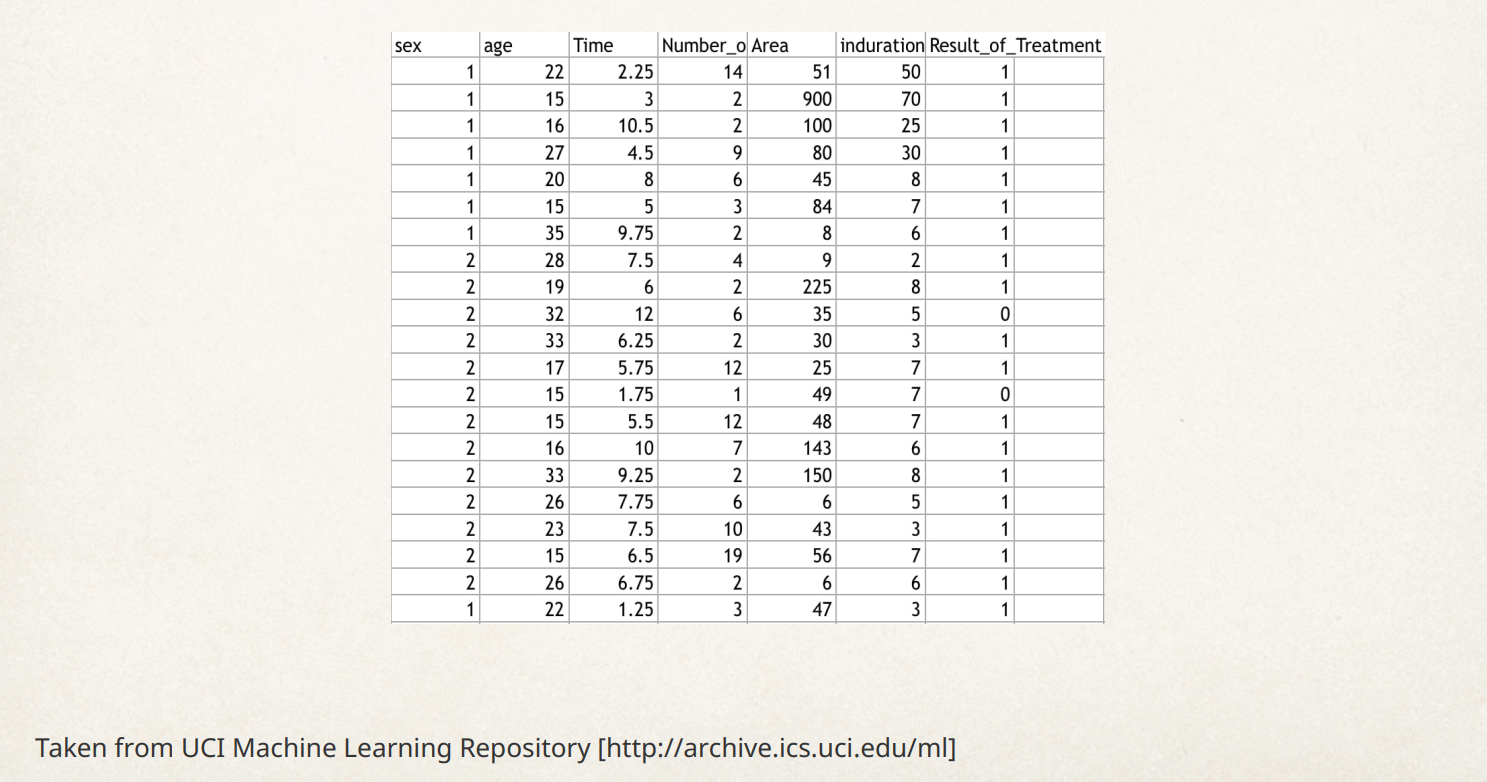
\includegraphics[scale=0.3]{chapters/pac/figures/ImmunotherapyDataSet.png}
    \caption{Immunotherapy Data Set}
\end{figure}
\end{example}

Let us list the ingredients of a general problem of this type:

\begin{itemize}
 \item The individual object, $\mathbf{x}$, that we wish to label. In our case, each such object is a vector $\mathbf{x}$ of $d$ real numbers describing $d$ features of a patient, as shown in the figure.
 \item The set of all possible $\mathbf{x}$'s is called the \textit{\textbf{Domain set, $\Xc$}}. We can take, for example,  $\Xc= \mathbb{R}^d$ (We could also take a smaller $\Xc$ since age must be positive and sex can have only two values).
 \item \textit{\textbf{Label set, $\Yc$}}: set of possible labels. In our case we can take, for example,  $\Yc=\{0,1\}$, where $0$ corresponds to a recommendation for not giving the treatment and 1 for giving it.
 \item \textit{\textbf{A prediction rule}}, $h:\Xc\to \Yc$: used to label future examples. This function is also called a \textit{\textbf{predictor}}, a \textit{\textbf{hypothesis}}, or a  \textit{\textbf{classifier}}.
\end{itemize}


The learner, that is, our algorithm, $\mathcal{A}$, receives an input, called the \textit{\textbf{Training data}},  which consists of $m$ already-labeled objects {$S=((\mathbf{x}_1,y_1),...,(\mathbf{x}_m,y_m)) \in  (\Xc\times \Yc)^m$. In our example, $m=21$ and these objects are the 21 lines in the figure. The learner's output is the prediction rule, $h:\Xc\to \Yc$. So a learner is a map $\mathcal{A}:S\mapsto h$. 
The learner's task is to produce an $h$ that will be sufficiently correct when labeling future objects, where  'sufficiently' should be clearly defined. If, for a large enough training data, the learner can always come up with such an $h$, we say that the task is \textit{learnable}.


\section{A Theoretical framework for learning}

The basic questions in machine learning are: Which tasks are learnable?  
How do we learn learnable tasks? How many training samples do we need in order to learn them? 
In this chapter we develop the \textit{\textbf{ PAC theory of learning}}, a famous theory that gives, within its definitions and assumptions, a complete answer to these questions,  for \textit{\textbf{ batch supervised learning}} ('batch', meaning that the whole training data set is fed at once into the algorithm and 'supervised' meaning that this set contains the labels, $y$, and not only the domain set, i.e., the $\mathbf{x}$ values ). \textcolor{blue}{[Was batch learning defined earlier?]}.

\subsection{A Data-generation Model }
From now on, we will use the following two assumptions:
\begin{itemize}
	\item There exists a (deterministic) function $f$ which is the correct classifier, i.e., for every $\mathbf{x}$ there is a single correct label, given by $y=f(\mathbf{x})$. We shall refer to this case as the \textit{\textbf{PAC Model}}.  In contrast, a bit later, we will consider a more general case which we will call the \textit{\textbf{Agnostic PAC model}} and in which the \textit{same} $\mathbf{x}$ may appear with \textit{different} labels, even within the same training set.
	
	
	\item All $\mathbf{x}$'s, both those that appear in the training set \textit{and} those in any future test set,  are independent and identically distributed (i.i.d) random variables, i.e., they are sampled independently using a distribution $\Dc$ over the example space $\Xc$. In particular, this means that the probability, $\Prob(S)$, of getting the sequence  $S=(\mathbf{x}_1,y_1),...,(\mathbf{x}_m,y_m)$ is given by $\Prob(S)=\prod_{i=1}^{m}\Dc(\mathbf{x}_i)$.   $\Prob(S)$ does not  depend on the labels $y_i$'s, since, by the previous assumption, these labels are uniquely determined by the $\mathbf{x}_i$'s and $f$. 
\end{itemize}




Compare the above PAC model to the first learning problem we saw, namely, the Linear Model. There, we also were given $m$ examples, $\mathbf{x}_1,..,\mathbf{x}_m\in\Xc$ (where we specifically took  $\Xc=\mathbb{R}^d$) but all of them received equal importance, for example, in their contribution to the global error (the loss function). Now, the examples $\mathbf{x}_i$'s are  i.i.d samples chosen according to $\Dc$, i.e., they have different probabilities to appear and therefore may have different weights in the loss function. Another difference is that in the case of the linear model we started with the assumption $y_i=f(\mathbf{x}_i)$ where $f$ was deterministic and linear. Here, we do assume $f$ to be deterministic, but otherwise it may take the form of any possible function from $\Xc$ to $\Yc$.
In the linear model we eventually relaxed the deterministic assumption and considered $y$ to be a random function of $\mathbf{x}$ of the form:  $y_i = f(x_i)+z_i$. 
An analogous generalization will take place also here, once we consider the more general, agnostic, case. Finally we note that, although this chapter will focus on \textit{classifiers}, many principles we will encounter will hold also for linear regression problems.

\subsection{Generalization Error for Classifiers}

For a classification task, we define the \textit{\textbf{Generalization Error}} of a hypothesis $h$ as the probability to obtain an $\mathbf{x}$ for which $h(\mathbf{x})$ is different than the correct label $f(\mathbf{x})$:
\[
L_{\Dc,f}(h) ~\equiv~ \Prob_{x \sim \Dc}[h(x) \neq f(x)] ~\equiv ~ \Dc\left( \{ x \in \Xc : h(x)
\neq f(x) \}\right) ~
\]
where $\Dc$ and $f$ are unknowns. The generalization error is also called the \textit{\textbf{risk}}, or the \textit{\textbf{true error}}. 
%Recall that $\Dc$ is a distribution over $\Xc$, that is, for a given $A \subset \Xc$, the value of $\Dc(A)$ is the probability to see some $x \in A$.

{\bf Note:} One should be critical about an error measure that counts the total number of misclassification errors of a classifier. Recall that  there are two kinds of errors a classifier can make: Type-I and Type-II errors, and one is usually much worse than the other. For now, we only note that, assuming $\Yc =\{0,1\}$, in the above definition of the true error, $h(x) \neq f(x)$ may refer either to  $h(x)=1, f(x)=0$ or to $h(x)=0, f(x)=1$ where one of these two cases  will correspond to a \textit{\textbf{False Positive}} event and the other to a \textit{\textbf{False negative}} event.
	


\subsection{Basic Definitions} \label{sec:frame}

Let us summarize the theoretical framework we have developed so far. Our task is to design a learning algorithm (a learner), $\mathcal{A}$. For a given sample size $m$, $\mathcal{A}$  takes a training sample $S=((\mathbf{x}_1,y_1),..,(\mathbf{x}_m,y_m))$ and outputs a prediction rule (a hypothesis)  $h: \mathcal{X}\to\mathcal{Y}$. 
For classification problems, $\mathcal{Y}=\{\pm 1\}$, but the framework we develop has a much broader applicability. 

We assume that the data points, both in training set and in the test set, are  generated by sampling independently $\Xc$ using a distribution  $\mathcal{D}$, which is unknown to us. The labels $y$ are fixed: all occurrences of a particular $\mathbf{x}$  will always be accompanied by the same label, $y=f(x)$, where $f$ is a deterministic function, which, like $\Dc$, is unknown to us (except for its values at the training data points: $ f(x_i)= y_i $, $i=1,\ldots,m$). Finally, the performance of any candidate rule $h:\mathcal{X}\to\mathcal{Y}$ that our learner may produce,  will be evaluated using by how well it will perform on future, unseen, samples - using the expected misclassification rate $L_{\Dc,f}(h) ~\equiv ~ \mathbb{P}_{x \sim \Dc}[h(x) \neq f(x)] \,.$

The following sections will be devoted for a detail understanding of the following important definitions.

\begin{definition} \label{PAC Learnable}
	A hypothesis class $\Hc$ is \textit{\textbf{ PAC Learnable}} if there exists a function $\tilde{m}_\Hc : (0,1)^2 \to \N$ and a learning algorithm $\Ac$ with the following property:
	For every $\epsilon,\delta \in (0,1)$ and for every distribution $\Dc$ over $\Xc$, and for every labeling function $f:\Xc\to\{\pm 1\}$ that satisfies $L_{\Dc,f}(h^*)=0$ for some $h^*\in\Hc$, when running the learning algorithm $\Ac$ on $m\ge \tilde{m}_\Hc(\epsilon,\delta)$ i.i.d. examples generated by $\Dc$ and labeled by $f$, the algorithm returns an hypothesis $h_S=\Ac(S)$ such that, with probability of at least $1-\delta$ (over the choice of the training samples), we have
	$
	L_{\Dc, f}(h_S) \le \epsilon
	$. 
	For a PAC learnable hypothesis class, we define the \textit{\textbf{ Sample  Complexity}} of $\Hc$ for specified $\epsilon,\delta$ as the minimal number of
	samples $\tilde{m}_\Hc(\epsilon,\delta)$ required for the definition to hold
	with respect to $\epsilon,\delta$. The Sample Complexity function of $\Hc$ is
	denoted $m_\Hc:(0,1)^2\to\mathbb{N}$.
\end{definition}

\begin{definition} \label{VC-dimension}
	Let $\Hc\subset\left\{ \pm 1 \right\}^\Hc$ be an hypothesis class.
	For a subset $C\subset \Xc$ let $\Hc_C$ be the restriction of $\Hc$ to $C$, namely,
	$\Hc_C = \{ h_C : h \in \Hc\}$, where for $h:\Xc\to\Yc$, $h_C:C\to\Yc$ is the
	function such that $h_C(x)=h(x)$ for every $x\in C$. Define the \textbf{\textit{ VC-dimension}} of $\Hc$ by
	\[
	VCdim(\Hc) := \max\{ |C| ~\Big|~ C\subset\Xc \,\,\text{and}\,\, |\Hc_C|=2^{|C|} \}
	\,.
	\]
	
	Note that $VCdim(\Hc)\leq \infty$. 
\end{definition}


\subsection{The Fundamental Theorem of Statistical Learning}

Definitions \ref{PAC Learnable} and \ref{VC-dimension} are interesting since, if we choose PAC learnability as our
interpretation of what learnability means, then we have a \textit{well defined necessary and sufficient condition for when it is possible to learn, in terms of the VC-dimension,  an exact minimal  training sample size we need in order to learn, and a "universal" learner that successfully learns when enough training data is available.} In short, we have a full theory of batch learning - a full theory of when it is possible to generalize from a training sample to new samples, and how to do it.
\vspace{3mm}
This result is sometimes known as ``\textit{\textbf{The Fundamental Theorem of Statistical Learning}}'' and states the following (roughly):
\begin{itemize}
	\item An hypothesis class $\Hc$ is PAC-learnable \textit{if and only} if
	$VCdim(\Hc)<\infty$
	\item The sample complexity of a hypothesis class with a finite VC-dimension is
	given approximately by\[
	m_H(\epsilon,\delta) \sim \frac{VCdim(\Hc)+\log(1/\delta)}{\epsilon}
	\]
	\item The ERM rule achieves this minimum, namely, when learning is possible, ERM
	learns with a minimial number of examples.
\end{itemize}

In the following sections, we will inspect the definitions of PAC-learnability and VC-dimension in great detail but in order to do so, let us first  present a different perspective of the framework we introduced in Section \ref{sec:frame}.

\subsection{Learning as a Game - first attempt}

The framework in Section \ref{sec:frame} can be thought of as a \textit{game} between us and Nature, with a random payoff. The game proceeds as follows. The number of training samples $m$ is given in advanced as a game parameter. \\

We move first. We choose a learner $\mathcal{A}$ that trains on $m$ samples. This is our strategy.
Nature moves second. Nature chooses a distribution $\mathcal{D}$ and a labeling function $f$. This is Nature's strategy. Importantly, Nature knows the strategy we chose when she chooses her strategy.
To calculate the game's payoff, an i.i.d sample $S$ of length $m$ is drawn according to the distribution $\mathcal{D}$ that Nature chose, is labeled according to the function $f$ that Nature chose, and is fed into the learner $\mathcal{A}$ that we chose to obtain the prediction rule $h_S:=\mathcal{A}(S)$ (the notation $h_S$ helps us remember that the prediction rule we learn, $h_S$, strongly depends on the random sample $S$ that we drew). The payoff is $L_{\Dc,f}(h)$. Our goal in the game is to end up with an $L_{\Dc,f}(h)$ which is as small as possible while Nature is an adversary that wants it to be as large as possible. Note that the payoff is random as it depends on the sample $S$ that was drawn. If we're unlucky, and the sample $S$ is "bad", namely, does not represent $\mathcal{D}$ very well, then the rule $h_S$ our learner produces might not generalize well and the random loss (for that draw of $S$) will be high. 

Now you might ask: what's the best strategy for us (how to best design $\mathcal{A}$)? 
Remember that Nature will know what we chose, and can try to be "cruel", namely, to choose $\Dc$ and $f$ that our learner did not prepare well for. Also, there's always a chance that we will draw a "lousy" sample $S$, namely a misleading sample that will confuse our learner and will cause it to output a rule $h_S$ that will not generalize well. Is there a way to "defend" ourselves against "cruel" strategies $\mathcal{D},f$ that Nature might play, and against "unlucky" draws of a training sample $S$? Is there anything at all that can be said in this generality about the problem of learning (i.e., the problem of generalizing from training samples to new samples)? 

\vspace{3mm}
\begin{definition}
Let's define this as \textit{\textbf{ The Learning Game}} (first version):
\begin{itemize}
	\item A sample size $m$ is fixed.
	\item We choose a strategy (a learner) $\Ac$, that is, a function that matches every sample $S \in (\Xc,\Yc)^m$ to a prediction rule $h_s \in \Yc ^\Xc$ 
	(which, by itself is a function, $h_S:\Xc\to\Yc$) 
	\item Nature knows our strategy, and, after us, chooses a strategy that consists of a probability distribution $\Dc$ over $\Xc$, and a label function $f:\Xc\to\Yc$. 
	\item A sample $S$ of size $m$ is drawn according to $\Dc$ and is labeled
	according to $f$
	\item The sample $S$ is fed into $\Ac$ to produce a prediction rule
	$h_S=\Ac(S)$
	\item The payoff is $L_{\Dc,f}(h_S)$, namely, the expected fraction of misclassification errors $h_S$ will make on data drawn i.i.d according to $\Dc$ and labeled according to $f$.
 The payoff is \textit{random} since $S$ is random and therefore $h_S$ is random.
	\item We are going to assume Nature is ``cruel'' and does her best to win.
	So we'll look for learners $\Ac$ for which we can \textit{ensure} that the loss $L_{\Dc,f}(h)$ never exceeds a certain value, \textit{for any} strategy $\Dc,f$ that Nature might play.
\end{itemize}
\end{definition}



\section{Probably correct \& Approximately correct learners}

\begin{definition} \label{approximately correct}
Let $0<\epsilon<1$.  We  say that a learner $\Ac$ is \textit{\textbf{Approximately Correct}}  with  \textit{\textbf{accuracy}} $\epsilon$, if we are certain (with probability 1) that for any training sample, $S$, drawn using $\Dc$, $\Ac$ will output a prediction rule, $h_S$, with a loss smaller or equal to $\epsilon$:
$$D\{S|~ L_{\Dc,f}(h_S) \leq \epsilon\}=1$$

Note that the loss is random - it depends on the draw of $S$ - therefore it makes sense to talk about the probability that a learner has a certain loss (a probability that, in the present case, is required to be 1).
\end{definition}

Now can ask the following question.
 
\textbf{Question}: Is there an accuracy parameter, $0\leq\epsilon<1$, for which we can choose a learner, $\Ac$,  that will be approximately correct? 
In other words, that almost surely (with probability 1), for any sample $S$ drawn according to $\Dc$, we will have  $L_{\Dc,f}(h_S) \leq \epsilon$?

\textbf{Answer}: {\bf No.} 
Choose $0\leq \epsilon <1 $. The learner cannot hope to produce, regardless of how Nature plays, and with probability $1$, a rule $h_S$ with $L_{\Dc,f}(h_S) \leq \epsilon$.
There's always a (small) probability to get a completely ``pathological'' training	sample $S$ that does not represent $\Dc$ at all. The resulting rule $h_S$ can
	be wrong on most of $\Xc$. If $S$ is really bad, $h_S$ can have a loss as high as $1$, higher than any $\epsilon$.
	
\begin{example}\label{counter example absolute confidence}

		Choose an accuracy $0\leq \epsilon <1 $. Take $\Xc=\left\{ x_1,x_2 \right\}$. 
		Our learner $\Ac$ must specify what to predict on a point that was not seen in the training set. 
		Let us consider the case where $S$ contains only $x_2$'s and denote it by $S_2$, that is, $S_2\equiv (x_2,f(x_2)), (x_2,f(x_2)),..., (x_2,f(x_2))$, 
		and assume, without a loss of generality, that in this case our algorithm predicts the label $x_1$ by $+1$:  $h_{S_2}(x_1)=+1$.
		Now, Nature chooses $\Dc$ with	$\Dc(\{x_1\}) = \gamma$, $\Dc(\{x_2\}) = 1-\gamma$, where $\gamma$ is a number satisfying  $0<\epsilon<\gamma<1$. 
		Nature also chooses a labeling function $f$ with  $f(x_1)=-1=-h_{S_2}(x_1)$. 
		So in case obtaining  $S_2$ as the training set,  the loss, $L_{\Dc,f}(h_{S_2})$ would satisfy
		$$L_{\Dc,f}(h_{S_2})>\gamma>\epsilon$$ 
		since the probability of drawing $x_1$ as a test point (on which Nature made sure that our prediction will fail)  is $\gamma$, and  $\gamma$ was chosen by Nature to be bigger than $\epsilon$. The probability of obtaining $S_2$ is $(1-\gamma)^m$, even if very small,  is not zero because $\gamma<1$ and therefore we failed to ensure with probability 1, that the loss will be smaller than $\epsilon$.  
		
		 
Thus, even on a sample space $\Xc$ with only two points, for any fixed $\epsilon>0$, for every strategy $\Ac$ we might play, Nature has a strategy $\Dc,f$, such that 
		with some probability over the choice of training samples of length $m$, we have  $L_{\Dc,f}(h_S) \geq \epsilon$. As $\epsilon$ was arbitrary, this means that for any arbitrarily "bad" loss $\epsilon$, Nature can, with non-vanishing probability,  cause the game to end with a loss of at least $\epsilon$.
	  What went wrong? In this example, with probability $(1-\gamma)^m$ (which can be really very tiny if $m$ is large) we get a "lousy" training sample, $S_2$, that does not represent $\Dc$  good enough, and does not allow us to generalize. 
  \end{example}
	  \vspace{3mm}
 
We therefore conclude that, given any accuracy parameter $0< \epsilon<1$, no learner $\Ac$ can guarantee, that with probability $1$, the loss will not exceed  $\epsilon$:  Nature can always find a strategy for which  $L_{\Dc,f}(h_S) > \epsilon$ will have a non-zero probability to occur. 

So now that we are aware that "bad" samples may always appear, with non-zero (even if small) probability, we should not aspire for an absolute certainty in achieving a limited loss. We will accept the fact that on these bad, but with limited chance to appear, training samples, the learner $\Ac$ might  "fail completely"	(produce $h_S$ with potentially huge loss).  We will, from now on, only require a limited certainty, that we will call 'confidence', for having a limited loss. This means that we will demand that the probability of drawing a bad sample will not exceed a certain threshold, that we will denote by $\delta$ and that  $\delta$ will be  specified in the initial parameters of the game, together with $\epsilon$. 

Since we no longer demand absolute confidence in having a limited loss, perhaps we can instead require absolute accuracy (zero loss), but with a limited confidence? 
That is, perhaps we can require that at least for those good training samples (the ones that will have a probability of $1-\delta$ to appear) the loss will vanish? 
 

\begin{definition} \label{probably correcty}
Let $0<\delta<1$. 	We  say that a learner, $\Ac$, is \textit{\textbf{Probably Correct}} with \textit{\textbf{confidence}} $\delta$, if the probability to obtain a training sample, $S$, for which $\Ac$ will output a prediction rule, $h_S$, with a perfect accuracy (zero loss), is larger or equal to $1-\delta$:
$$D\{S|~ L_{\Dc,f}(h_S)=0\}\ge 1-\delta$$
  
Note that in definition \ref{approximately correct}  we required  prefect confidence $\delta=0$ ("with probability 1" ), to have a certain accuracy ($\epsilon<1$),
while in definition \ref{probably correcty}  we require a certain confidence $\delta<1$ to have a prefect accuracy $\epsilon=0$. 
\end{definition}
Definition \ref{probably correcty} helps us rephrase the  question above more formally.
 

\textbf{Question:} Is there a confidence parameter  $0<\delta<1$,  for which we can choose a learner, $\Ac$, that will be probably correct?
In other words, in the event of a non-pathological sample (the event with probability of at least $1-\delta$) can we achieve perfect accuracy,  $L_{\Dc,f}(h_S) = 0$?  

\textbf{Answer:} {\bf No.} Choose $0<\delta<1$. The learner cannot 	hope to produce, with probability of at least $1-\delta$, a rule $h_S$ with $L_{\Dc,f}(h_S)=0$, independently of how Nature plays.  $L_{\Dc,f}(h_S)=0$ means that $\Dc\{h_S(x)= f(x)\}=1$ ($h_S$ is, with probability 1 with respect to $\Dc$, always correct). 	Nature can choose some $x\in\Xc$ and can play a $\Dc$ that gives a finite but tiny probability mass to a certain $x$. Then, with high probability, the sample $S$ will not include $x$, and therefore, whatever label the learner assigns to $h_S(x)$, it will be a guess and therefore might be incorrect, causing a finite loss.
	
\begin{example} \label{counter example absolute accuracy}
	Choose a confidence $0<\delta <1$. Take $\Xc=\left\{ x_1,x_2 \right\}$. 
	
	As in example \ref{counter example absolute confidence} , we consider the case of the training sample $S_2\equiv (x_2,f(x_2)), (x_2,f(x_2)),..., (x_2,f(x_2))$. 
	Once again we assume that in this case our algorithm predicts the label $x_1$ by $+1$:  $h_{S_2}(x_1)=+1$.
	As in example \ref{counter example absolute confidence}, Nature chooses a labeling function $f$ with  $f(x_1)=-1=-h_{S_2}(x_1)$ and a distribution, $\Dc$, with	$\Dc(\{x_1\}) = \gamma$, $\Dc(\{x_2\}) = 1-\gamma$, but now $\gamma$ is chosen so that  $\delta<(1-\gamma)^m$. Note that this requirement means that when $m$ is large, Nature chose the probability of getting $x_1$, namely, $\gamma$, to be close to zero, which means that $S_2$ is actually a typical ("non-pathological", "good") sample: its probability to appear, $(1-\gamma)^m$ is larger than $\delta$.
	
	As in example \ref{counter example absolute confidence}, in case of obtaining  $S_2$ as the training set,  the loss, $L_{\Dc,f}(h_{S_2})$ would satisfy
	$$L_{\Dc,f}(h_{S_2})>\gamma$$ and since $\gamma>0$ that would mean a non-zero loss. 
  Since $S_2$ has a probability $(1-\gamma)^m$ to appear and since $(1-\gamma)^m >\delta$, the probability of ending up with a non-zero loss is larger than $\delta$.
  In other words, our learner $\Ac$ is not a probably correct one. 
\end{example}
	
	We conclude that for any confidence parameter  $0<\delta<1$, no learner $\Ac$ can guarantee, that with probability $1-\delta$, the loss will vanish: Nature can always find a strategy for which $L_{\Dc,f}(h_S) > 0$ will have a probability large than $\delta$ to occur. Even a "typical"  training sample may miss small areas in $\Xc$. On these areas
	the resulting $h_S$ might be wrong. We have to allow $h_S$ to be wrong sometimes (to make some generalization errors) even when the training sample is "typical".
	
	So whatever learner we construct, we can never have an absolute confidence that our loss limited by some fixed $\epsilon$, neither we can have even a limited-confidence (with probability larger than  $1-\delta$, for some fixed $\delta$) in obtaining an absolute accuracy. 	What we might be able is to have is a limited-confidence that our loss will be limited, which brings us to the following definition.
	
\begin{definition}	
	Let $\delta>0$ and $\epsilon>0$. We say that a learner, $\Ac$, is \textit{\textbf{Probably Approximately Correct}} with a confidence $\delta$ and an accuracy $\epsilon$ if the probability of obtaining a training sample, $S$, for which $\Ac$ will output a prediction rule, $h_S$, with a loss that does not exceeds $\epsilon$, is larger or equal to $1-\delta$:
		$$D\{S|~ L_{\Dc,f}(h_S)=0\}\ge 1-\delta.$$
\end{definition}


%With the above formal framework, the following questions can be formulated mathematically.

%\begin{itemize}
% \item Can we find $h$ with $L_{\Dc,f}(h) = 0$
%\item Can we find such "good" $h$, no matter what $S$ is?
%\item Can we find such "good" $h$, no matter what $\Dc$ is?
%\item Can we find such "good" $h$, no matter what $f$ is?
%\item How big should $m$ be?
%\end{itemize}

It is important to understand the difference between the  \textit{accuracy}  $\epsilon$ and the \textit{confidence} $\delta$:
\textit{First}, we draw the training sample $S$ at random. The learning algorithm runs on this random input and its prediction is therefore random.
If $S$ is by chance "weird" (not representing $\Dc$ well), the rule $h_S$ produced will be "wrong", namely, it won't generalize well. The number $\delta$ is the probability of failure due to a "weird" sample $S$. \textit{Second}, we test the rule $h_S$ on new data. The new data is also random. $L_{\Dc,f}(h_S)$ is  the expected number of errors $h_S$ will make, i.e., its accuracy. The number $\epsilon$ refers to that accuracy.

\subsection{The game - for Probably Approximately correct learners}

Since we can only hope to build a Probably Approximately correct learner, we
will update the game definition a little. The sample size $m$ will no longer be
fixed. Instead, the accuracy $\epsilon$ and confidence $\delta$,  which our
learner is required to achieve, are specified as game parameters. We get to
decide on $m$ in our strategy. Note that there is subtle nuance in notation now:
when we write $\Ac$ for the learner, we actually mean a {\bf sequence} of
learners - one for each $m$. It would be better to write $\Ac_m:(\X\times \Yc)^m
\to \Yc ^\Xc$, but we won't bother writing $\Ac_m$ and will continue to use $\Ac$.
\vspace{3mm}
So here is our updated game - The Learning Game (second version): Fix desired accuracy $\epsilon>0$ and confidence $\delta>0$. We play a game against Nature, with random payoff.
\begin{itemize}
	\item We choose a sample size $m$ and a learner $\Ac:(\Xc,\Yc)^m \to \Yc ^\Xc$. 
	Both $m$ and $\Ac$ can depend on $(\epsilon,\delta)$.
	\item Nature knows our strategy, and, after us, chooses strategy that consists of a probability distribution $\Dc$ over $\Xc$, and a label function $f:\Xc\to\Yc$. 
	That is, Nature's strategy can depend on $(\epsilon,\delta)$ specified, and also on the $m,\Ac$ we chose. 
	\item A sample $S$ of size $m$ is drawn according to $\Dc$ and is labeled
	according to $f$
	\item The sample $S$ is fed into $\Ac$ to produce a prediction rule
	$h_S=\Ac(S)$
	\item The payoff is $L_{\Dc,f}(h_S)$. It is random since $S$ is random and
	therefore $h_S$ is random.
	\item We are going to assume Nature is ``cruel'' and does her best to win.
	So we'll look for learners $\Ac$ that have a {\bf guaranteed maximal 
		loss} $L_{\Dc,f}(h)$ {\bf for any} strategy $\Dc,f$ that Nature might play.
	\item To determine if we were successful in the game, we play the game many many times 
	(both us and Nature play the same strategies, just the training samples drawn are different).
	We count and calculate the probability, over the random draws of training samples $S$, of the event
	$\{ S \sim \Dc ^m \,\big |\,L_{\Dc,f}(h_S)\leq \epsilon \}$. If this probability is found to be 
	larger than $1-\delta$, that is, if 
	the learner $\Ac$ we chose was Probably Approximately correct with accuracy $\epsilon$ and confidence $\delta$ - against Nature's best strategy - {\bf we say that we've been successful (with regards to the parameters $\epsilon,\delta$)}.
\end{itemize}


If you don't like the game perspective, here our current definition of our learning challenge:
The learner doesn't know $\Dc$ and $f$. The learner receives an accuracy parameter $\epsilon$ and a confidence parameter $\delta$. It then ask for training data, $S$, containing $m(\epsilon,\delta)$ examples (that is, the number of examples can depend on the value of $\epsilon$ and $\delta$, but it can not depend on the unknown $\Dc$ or $f$). Finally, the learner should output a hypothesis $h_S$, that depends only on $\epsilon, \delta$ and the training sample $S$ drawn, such that with probability of at least $1-\delta$  it holds that $L_{\Dc,f}(h) \le \epsilon$. That is, the learner should be Probably Approximately correct, with the specified accuracy $\epsilon$ and confidence $\delta$.

\vspace{3mm}
Since we can now choose the sample size $m$, and data costs money, we want $m$ to be as small as possible - as long as we still design a probably approximately correct learner. We sense that there must be some trade-off between $\epsilon,\delta$ and $m(\epsilon,\delta)$
The figure below shows schematically the connection between $m$,$\delta$, and $\epsilon$.

\begin{figure}[h!]
	\centering
	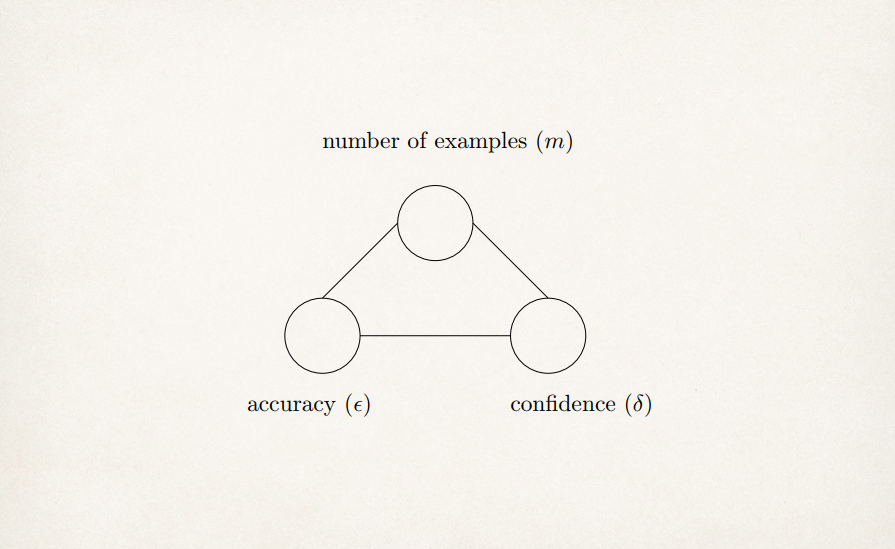
\includegraphics[scale=0.3]{chapters/pac/figures/m_eps_del.png}
	\caption{Connection between $m$,$\delta$, and $\epsilon$.}
\end{figure}


\section{No Free Lunch and Hypothesis Classes}


%\textcolor{blue}{We note again that the meaning of "with probability of at least $1-\delta$" is the probability with respect to the sample $S$.
%In other words, the probability of getting a sample $S$ that will cause the algorithm to output a not-accurate-enough $h$ should be smaller than $\delta$.}


\subsection{No Free Lunch!}

Turns out that, unfortunately, we cannot in general be successful against Nature even in this second version of our game - for any parameters $\epsilon,\delta$...
Why? If we know nothing about $D$ and $f$, and if there are too many possibilities for $f$, then no matter how large our sample size, $m$, we can not be confident-enough that we can find an accurate-enough $h_S$. Let's understand why.
\vspace{5mm}

The two examples above (which demonstrated we can't hope to get a learner that enjoys confidence $\delta=0$ or accuracy $\epsilon=0$) only needed a sample space $\Xc$ with two points. 
Now let's consider a sample space with a countably infinite number of points.  
\vspace{3mm}
{\bf Example.}
\begin{itemize}
	\item Suppose that $|\mathcal{X}| = \infty$. Recall that we move first and choose $m$, and that Nature knows the $m$ we chose. So, let our choice of $m$ be fixed. We must choose what to predict on a point we have not seen in the training sample. Denote our choice by 
	$g(x)$. That is, our learner $\Ac$ specifies that if a point $x\in\Xc$ was {\bf not} observed in our training data, then the rule that $\Ac$ outputs will predict $h_S(x)=g(x)$. 
	\item Now, Nature picks some finite set $C \subset \Xc$ with $ |C| > 2m$, and chooses $\Dc$ to be uniform 
	over $C$. For the labeling function $f$, Nature plays a sinister move, and chooses $f(x)=-g(x)$ for all $x\in\Xc$. (The opposite of what $h_s$ will predict on unseen points!)
	\item Now, let $S$ be a training sample. Let $supp(S)\subset C$ denote all points $x\in\Xc$ observed in the particular training sample $S$.
	Since $|supp(S)|\leq m$ and since $\Dc$ is uniform over $C$, we have $\Dc(\{x\in \Xc\setminus supp(S)\})\geq 1/2$.
	In other words, the probability that a new test point drawn according to $\Dc$ will be unseen in $S$ is at least $1/2$.
	\item Now, as the game demands, we feed the sample $S$ into $\Ac$ and obtain $h_S=\Ac(S)$. What is the loss? Regardless of what $h_S$ predicts on points in the training sample $S$, since a test point has probability $\geq 1/2$ to be in the unseen part $\Xc\setminus supp(S)$, with probability at least $1/2$, the rule $h_S$ will predict $h_S(x)=g(x)$ - and will be wrong, since Nature played the function $f(x)=-g(x)$. We conclude that, on the particular training sample $S$, we must have $L_{\Dc,f}(h_S)\geq 1/2$.
	\item But this happens for {\bf every} training sample $S$. So, Nature played a strategy for which, with probability $1$ over the choice of training samples (according to $\Dc$), the game results in loss  $L_{\Dc,f}(h_S)\geq 1/2$.
	\item So, if we were looking to find a learner $\Ac$ that will be Probably
	Approximately correct (to some specified $\epsilon$ and $\delta$ regardless of Nature's strategy $\Dc,f$, we find that we cannot. And asking for a larger training sample won't help - if we increase $m$, Nature will just choose a larger set $C$ and a distribution $\Dc$ uniform over that larger $C$.
	\item What went wrong? Nature could choose {\bf any labeling function at all} $f$ that she wanted, and we tried to learn (to generalize = to accurately predict) $f$ from a sample that was too small for the number of possible functions we needed to choose from. We find we just cannot design a Probably Approximately correct learner if the set of possible labeling functions is "too large". 
\end{itemize} 

\vspace{3mm}
This is known as a {\bf "No Free Lunch" Theorem}: without assuming anything in advance on $f$, without an prior information on the labeling function we are trying to learn, we find that learning is impossible. Equivalently, if the set of possibilities for the labeling function $f$ is too large, then Nature can be cruel and play a function that we can't learn - the larger the sample size we choose, the more complicated the function $f$ that Nature playes. So if the set of possibilities for the labeling function $f$ is too large, learning is impossible (in the sense of the game that we defined).
\vspace{3mm}
{\bf Important Note!} The argument given above is in fact wrong (can you find where?). While this was not a proof of a No Free Lunch Theorem, it gives all the crucial bits of intuition, and we will need them later. So we will call it a "proof" in quotes. 
\vspace{3mm}
Here is an actual, formal No Free Lunch theorem. (There are many theorems that can be called by that name - basically any theorem that shows that without some prior knowledge on the labeling function, when there are "too many" possibilities for $f$, learning it is impossible.) You can read the proof in  the Understanding Machine Learning book - Theorem 5.1, and exercise 3 in section 5.5. (it is not so easy to read and uses Agnostic PAC, a notion we will only get to later.) 


\begin{theorem}[No Free Lunch]
	$\Xc$ be an infinite sample domain, $|\Xc|=\infty$. Fix $\epsilon < 1/2$. There always exists some $\delta>0$ so that, for every learner $\Ac$ and training set size $m$, there exists a distribution $\Dc(x)$ over $\Xc$ and a function  $f:\Xc\to\Yc$, such that with probability of at least $\delta$ over the generation of a training sample $S$ of size $m$ drawn i.i.d from $\Dc$, we have
	$L_{\Dc,f}(h_S) \ge \epsilon$ where $h_S=\Ac(S)$.
\end{theorem}

%As a result we can conclude the following:
%\begin{theorem}[No Free Lunch (2)]
%Let $\Xc$ be an infinite domain set and let $\Hc$ be the set of all functions from $\Xc$ to $\{0,1\}$.
%for \textit{any} algorithm, there exist $D(x)$, $f$ and there exists at least some $0<\epsilon,\delta < 1$ so %that the probability of receiving an $S$ with $L_{\Dc,f}(A(S)) \ge \epsilon$ is larger than $\delta$.
%In such a case  we say that "H is not \textbf{PAC learnable}" (we will repeat the definition of PAC learnability %below).
%\end{theorem}

%\color{black}
%\pause
%\textbf{Remark}: $L_{\Dc,f}(\text{random guess}) = 1/2$, so the theorem
%states that you can't be better than a random guess
%\begin{center}
%  Please read the proof in {\em Understanding Machine Learning} ch. 5.1 \textcolor{blue}{and the exercises at %the end of ch. 5. Note that although the theorem in the book consider the case where $D=D(x,y)$ is a joint %probability of $x$ and $y$ (a situation we will discuss in the next lecture) the proof applies also to the case %where $D=D(x)$. }.
%\end{center}


\subsection{We need hypothesis classes}

So, in order to be able to learn, the learner {\bf must} receive enough prior knowledge about the function $f$.
This implies that we should assume that the target $f$ comes from some \textbf{hypothesis class}, $\Hc \subset \Yc ^\Xc$. 

\subsection{Realizability Assumption.} Suppose that an hypothesis class $\Hc$ is specified for our game. The {\bf realizable case} is when Nature must play a function $f\in\Hc$. Actually, we don't care if Nature plays a function $f$ that is not in $\Hc$ as long as $f$ is $\Dc$-almost surely identical to a function $h^*\in\Hc$.  (This is because we will never see samples in $\Xc$ where $f(x)\neq h(x)$ - not in the training and not in the test samples.) So the formal mathematical {\bf Realizability Assumption} is this: Nature plays a function $f$ such that there exists $h^*\in\Hc$ with $L_{\Dc,f}(h^*)=0.$
\vspace{3mm}
The learner is given $\Hc$ before learning starts, and will only output $h_S\in\Hc$. In other words, for a training sample of size $m$ the learner (learning algorithm) is a map $\Ac:(\Xc\times\Yc)^m\to\Hc$ such that $\Ac:S\mapsto h\in\Hc$. (As before, we will continue to abuse notation and write $\Ac$ instead of $\Ac_m$, and when we say "the learning algorithm $\Ac$" we will sometimes mean "a sequence of learners $\{\Ac_m\}_{m=1}^\infty$, one for each possible sample size").

\vspace{3mm}
We've just seen that if $|\Xc|=\infty$ then $\Hc   = \Yc ^\Xc$ is "too large to learn".
And, in a previous section we've seen that the learner gets to specify the training sample size $m$. 
The questions that arise now are:
\begin{itemize}
	\item What are the "small enough" hypothesis classes $\Hc$ for which we {\bf can} find a Probably Approximately correct learner?
	And what are the "too large" hypothesis classes $\Hc$ for which we {\bf cannot}? Can we characterize exactly the hypothesis classes for which it is possible to learn?
	\item Assume we have a "small enough" $\Hc$. This means that for every
	$\epsilon,\delta$ we have at least one strategy $m,\Ac$ such that $\Ac$
	is Probably Approximately correct (with accuracy $\epsilon$ and
	confidence $\delta$) no matter how Nature plays. This means that for
	every $\epsilon,\delta$ there is a {\bf minimal number of training
		samples}: maybe some learners are wasteful and need more training data
	than others, but for every $\epsilon,\delta$ there is the absolutely
	minimal training sample size that allows us to choose a Probably Approximately correct learner. Can we characterize this minimal function 
	$m_\Hc(\epsilon,\delta)$? Is there a connection between the "size" of the hypothesis class $\Hc$ and
	$m_\Hc(\epsilon,\delta)$?
	\item Assume we have a "small enough" $\Hc$. Can we characterize explicitly a learner $\Ac$ that always succeeds in learning functions from $\Hc$? And how many training samples $m$ does $\Ac$ need to always succeed in learning a function from $\Hc$ (always be Probably Approximately correct, no matter how Nature plays)? Can we find the {\bf most training-data efficient} learner, namely a learner that can succeed with the minimal number of samples $m_\Hc(\epsilon,\delta)$ mentioned above?
\end{itemize}


\subsection{Updating the game one last time}

So here is our final version of the game - ({\bf The Learning Game (third
	version):} Fix desired accuracy $\epsilon>0$ and confidence $\delta>0$. Fix
an hypothesis class $\Hc \subset \Yc ^\Xc$. 
We play a game against Nature, with random payoff.
\begin{itemize}
	\item We choose a sample size $m$ and a learner $\Ac:(\Xc,\Yc)^m \to \Hc$. 
	Both $m$ and $\Ac$ can depend on $(\epsilon,\delta)$.
	\item Nature knows our strategy, and, after us, chooses strategy that consists of a probability distribution $\Dc$ over $\Xc$, and a label function {\bf from the specified hypothesis class} $f\in\Hc$. 
	That is, Nature's strategy can depend on $\epsilon,\delta,\Hc$ specified, and also on the $m,\Ac$ we chose. 
	\item A sample $S$ of size $m$ is drawn according to $\Dc$ and is labeled
	according to $f$
	\item The sample $S$ is fed into $\Ac$ to produce a prediction rule
	$h_S=\Ac(S)$. Note that $h_S\in\Hc$.
	\item The payoff is $L_{\Dc,f}(h_S)$. It is random since $S$ is random and
	therefore $h_S$ is random.
	\item We are going to assume Nature is ``cruel'' and does her best to win.
	So we'll look for learners $\Ac$ that have a {\bf guaranteed maximal 
		loss} $L_{\Dc,f}(h)$ {\bf for any} strategy $\Dc,f$ that Nature might play.
	\item To determine if we were successful in the game, we play the game many many times 
	(both us and Nature play the same strategies, just the training samples drawn are different).
	We count and calculate the probability, over the random draws of training samples $S$, of the event
	$\{ S \sim \Dc ^m \,\big |\,L_{\Dc,f}(h_S)\leq \epsilon \}$. If this probability is found to be 
	larger than $1-\delta$, that is, if 
	the learner $\Ac$ we chose was Probably Approximately correct with accuracy $\epsilon$ and confidence $\delta$ - against Nature's best strategy - {\bf we say that we've been successful (with regards to the parameters $\epsilon,\delta$) and hypothesis class $\Hc$}.
\end{itemize}


\subsection{Example: Threshold functions}

%\textcolor{red}{[I modified a bit this section resolve the following issues:
%\textbf{a.} Sign function (as defined in python, wolfram) has three possible values {-1,0,+1} and therefore doesn't fit to a binary label (especially important when $\Xc$ is discrete). In any case, standard definition of threshold function (see e.g. Sec. 20.1 in UML) is: $f_{\theta}=\mathds{1}_{x>\theta}$ which is 0 for $x\leq %\theta$ and is 1 elsewhere.
%\textbf{b.}  $\theta'$ is not defined if $\Dc(\{x: -\infty < x < \theta\})=\epsilon$, (quite possible)
%\textbf{c.} The algorithm isn't well defined for the case $\theta < x_i$ for every $i$]}


We saw above that if $|\Xc|=\infty$ and $\Hc$ is the class of all functions from
$\Xc$ to $\Yc$, namely $\Hc=\Yc ^\Xc$, we can't be successful in the  the third version of the learning game. 
Well, maybe it's just impossible to learn when $|\Xc|=\infty$?  Fortunately, when the hypothesis class is "small enough", it \textit{is} possible to be successful in the third version of the learning game, which is the reason why learning is possible . In the following example we will have an infinite (in fact uncountably infinite) sample space, and a very simple hypothesis class. We will see that we can be successful in the third version of the game, for any $\epsilon,\delta$ specified. 

Consider the domain $\Xc=\mathbb{R}$, i.e., there is only one feature. We work with classification, and use the label set is $\Yc=\{0,1\}$ (instead of $\{+,-\}$).
Define the hypothesis class of \textbf{Threshold functions:}  over $\mathbb{R}$:
$$\Hc_{th} = \{ x \mapsto h_{\theta}(x) : \theta \in \R \ \bigcup \pm\infty\}$$
where $ h_{\theta}(x)=0$ for $x\leq \theta$ and $ h_{\theta}(x)=1$ for $x> \theta$. (We define $h_{\infty}(x)=0$ for all $x$, and $h_{-\infty}(x)=1$ for all $x\in\mathbb{R}$).

\begin{figure}[h!]
	\centering
	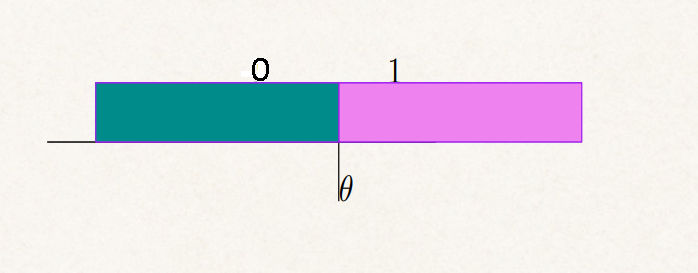
\includegraphics[scale=0.3]{chapters/pac/figures/threshold.png}
\end{figure}
\vspace{5mm}

What's the meaning of this definition? We are classifying points on the real line. Up until a certain unknown point, the points are in class $0$. Beyond that point, they are in class $1$. Nature chooses the true cutoff threshold $\theta$, and a distribution $\Dc$ over the real line.  We would like to receive a training sample $S$ of labeled points, and successfully predict the label of future examples. In this case, our job is to determine, as accurately as possible, the unknown cutoff $\theta$. (It is recommended to take some time and understand all the details of this example!) 

Now that we know our hypothesis class to be $\Hc_{th}$, we should specify our strategy, which consists of the number of samples $m$ we need, and a learning algorithm $\Ac$ that will process training sample and produce a decision rule. As before let $S=((x_1,y_1),...,(x_m,y_m))$ be the training set. As we will see, our choice of learner will not depend on the $\epsilon, \delta$ specified, but our choice of $m$ will certainly depend on them.

\subsubsection*{Learning algorithm}

Let's start with a suggested learning algorithm.
The training data may take the form shown in the three figures below, but not
the form shown in the fourth figure, which is forbidden because it does not obey
the Realizability Assumption (the assumption that Nature chooses $h\in\Hc$).

\begin{figure}[h!]
	\centering
	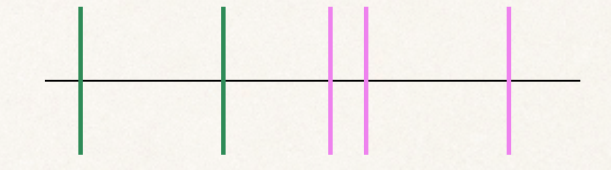
\includegraphics[scale=0.3]{chapters/pac/figures/thresholds1.png}
	\caption{Possible training data for $\Hc_{th}$}
\end{figure}

\begin{figure}[h!]
	\centering
	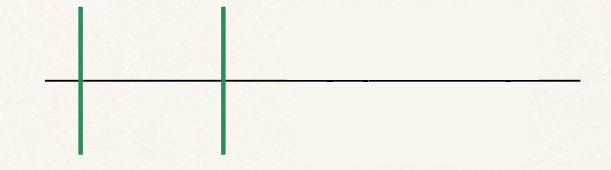
\includegraphics[scale=0.3]{chapters/pac/figures/thresholds1a.png}
	\caption{Possible training data for $\Hc_{th}$}
\end{figure}

\begin{figure}[h!]
	\centering
	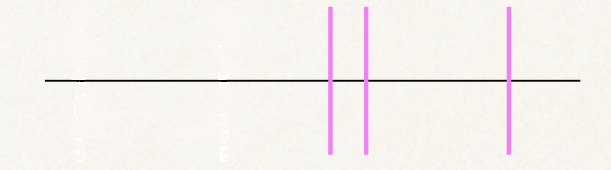
\includegraphics[scale=0.3]{chapters/pac/figures/thresholds1b.png}
	\caption{Possible training data for $\Hc_{th}$}
\end{figure}

\begin{figure}[h!]
	\centering
	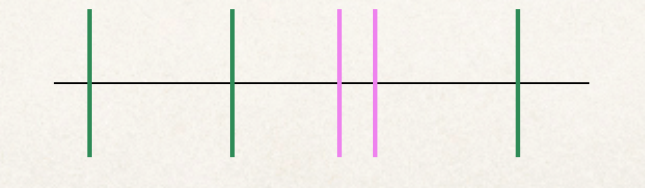
\includegraphics[scale=0.3]{chapters/pac/figures/thresholds2.png}
	\caption{Forbidden training data for $\Hc_{th}$ - violates the Realizability Assumption}
\end{figure}


We suggest the following learning algorithm: return hypothesis $h_{\theta_{alg}}(x)$ with $$\theta_{alg} = \max_{y_i=0} x_i$$.
If $y_i=1$ for all $i=1\ldots m$ then return $\theta_{alg} = -\infty$, namely, return a rule that classifies all points to $1$. Similarly, if $y_i=0$ for all $i=1\ldots m$ then return $\theta_{alg} = +\infty$, namely, return a rule that classifies all points to $0$.

\vspace{5mm}

\subsubsection*{Number of Samples}

Let $0<\epsilon,\delta$ be the accuracy and confidence specified in the game.
What should be out choice of $m$? Namely, how many samples are needed to guarantee that the true error is at most $\epsilon$ with probability at least $1-\delta$?

\begin{claim}
	Fix $0<\epsilon,\delta$.
	If $m \ge \frac{\log(1/\delta)}{\epsilon}$ then for any distribution $\Dc$ over the real line, and any choice of  labeling threshold function $f_\theta \in \Hc_{th}$,  with probability of at least $1-\delta$ (over the choice of training sample $S$ of size $m$), the loss
	$L_{\Dc,\theta}(h_{\theta_{alg}})$
	of the algorithm for learning threshold functions is at most $\epsilon.$
\end{claim}

\textbf{Proof}:
Fix distribution $\Dc$ over the domain set. Fix correct hypothesis $f_{\theta}\in \Hc_{th}$.

\begin{figure}[h!]
	\centering
	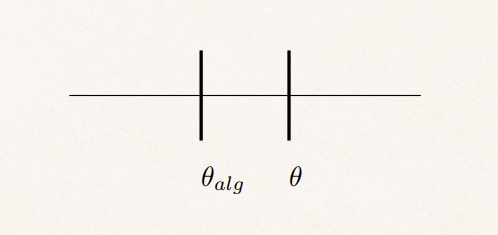
\includegraphics[scale=0.3]{chapters/pac/figures/thresholds3.png}
\end{figure}


From the properties of the algorithm we know that:
$$\theta_{alg} < \theta$$
Note that the prediction rule produced by the algorithm will be correct for test samples $x<\theta_{alg}$ and $x>\theta$ and is incorrect for $\theta_{alg}<x<\theta$.

\vspace{5mm}

If $\Dc(\{x: -\infty < x < \theta\})<\epsilon$  then $\Dc(\{x: \theta_{alg} < x < \theta\})<\epsilon$  and therefore the true error is \textit{always} (that is, with probability 1, no matter what $S$ or $m$ is) smaller than $\epsilon$ and we are done. We will therefore assume that $\Dc(\{x: -\infty < x < \theta\})\geq \epsilon$  and define $\theta'$ such that $\Dc(\{x: \theta' < x < \theta\})=\epsilon$.
\begin{figure}[h!]
	\centering
	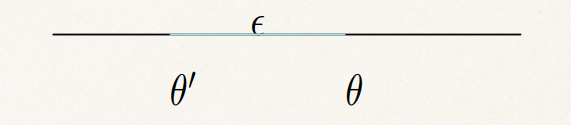
\includegraphics[scale=0.3]{chapters/pac/figures/thresholds4.png}
\end{figure}
\vspace{3mm}
Note that if there is $(x, y)\in S$ with $\theta'\leq x\leq\theta$ then the true error is at most $\epsilon$ and the probability not to get such a test sample is $(1-\epsilon)^m$.
Using  $1-\epsilon \le e^{-\epsilon}$, we see that the term $e^{-\epsilon m}$ would be smaller than $\delta$ if $m \ge  \frac{\log(1/\delta)}{\epsilon}$.


\subsubsection{Threshold functions - conclusion}

We saw that, for $\Xc=\mathbb{R}$, $\Yc=\{0,1\}$ and $\Hc=\Hc_{th}$ (the hypothesis class of threshold functions), we have a strategy (choice of sample size $m=m(\delta,\epsilon)$ and learning algorithm $\Ac$) that is {\bf always successful against Nature}, for any values $\epsilon, \delta$ specified. In other words, for any  $\epsilon, \delta$, our strategy (which depends on $\delta,\epsilon)$ specified) is a Probably Approximately correct learner regardless of how Nature plays. 
\vspace{3mm}
We recall that for $\Xc=\mathbb{R}$, $\Yc={0,1}$ and $\Hc=\mathbb{R}\to\mathbb{R}$ there were values of $\epsilon, \delta$ for which we {\bf could not be successful} regardless of how we played (in fact, we could not be successful for any $\epsilon<1/2$). So whether we can be successful for any values $\epsilon, \delta$ seems to be a property of the hypothesis class we choose. 
\vspace{3mm}
This brings us to the famous definition of a {\bf Probably Approximately Correct (PAC) learnable hypothesis class}.



\section{PAC learning}
\begin{definition}
	\begin{enumerate}
		\item
		A hypothesis class $\Hc$ is {\bf PAC Learnable} if there exists a function $\tilde{m}_\Hc : (0,1)^2 \to \N$ and a learning algorithm $\Ac$ with the following property:
		For every $\epsilon,\delta \in (0,1)$ and for every distribution $\Dc$ over $\Xc$, and for every labeling function 
		$f:\Xc\to\{\pm 1\}$ that satisfies $L_{\Dc,f}(h^*)=0$ for some $h^*\in\Hc$, when running the learning algorithm $\Ac$ on $m\ge \tilde{m}_\Hc(\epsilon,\delta)$ i.i.d. examples generated by $\Dc$ and labeled by $f$, the algorithm returns an hypothesis $h_S=\Ac(S)$ such that, with probability of at least $1-\delta$ (over the choice of the training samples), we have
		$
		L_{\Dc, f}(h_S) \le \epsilon
		$. 
		\item For a PAC learnable hypothesis class, we define the {\bf Sample Complexity} of $\Hc$ for specified $\epsilon,\delta$ as the minimal number of samples $\tilde{m}_\Hc(\epsilon,\delta)$ required for the definition to hold with respect to $\epsilon,\delta$. The Sample Complexity function of $\Hc$ is denoted $m_\Hc(0,1)^2\to\mathbb{N}$.
	\end{enumerate}
\end{definition}

Note that  PAC learnability is only one possible definition of learning that can account for the fundamental limitations on accuracy and confidence. We could, for example, settle for a specific, "good enough", values of $\delta$,  and $\epsilon$ instead of requiring that the condition that $m > m(\epsilon, \delta)$ implies  $L_{\Dc, f}(h) \le \epsilon$, to hold, for {\bf any} $\delta, \epsilon <1$.

\subsection{Finite hypothesis classes are PAC learnable}

In order to understand more about when PAC learning is possible (namely, which hypothesis classes are PAC learnable) let us first consider the case where $\Hc$ is a \textit{finite} hypothesis class.
Finite hypothesis classes can be huge: for example, take $\Hc$ is all the functions from $\Xc$ to $\Yc$ that can be implemented using a Python program of length at most $b$, for $b$ fixed and large. Or, take $\Hc$ to be all the functions from $\Xc$ to $\Yc$ where  $|\Xc|$ and $|\Yc|$ are finite.

\subsubsection{Empirical Risk Minimization}

You might expect that there would be nothing to say in this generality, namely,
that in order to design a successful learning algorithm we must pay attention to
the details of the specific $\Xc$ and finite $\Hc$ at hand.
Now comes a big surprise. It turns out that {\bf there is a simple learner that is always successful on finite hypothesis classes} (and on many other hypothesis classes as we will see later).

The idea behind this amazing learning is very simple and natural: try to be as correct as possible on the training data!

Formally, given  a training set $S = (x_1,y_1),\ldots,(x_m,y_m)$ we define the {\bf empirical risk} of a candidate prediction rule $h\in\Hc$ by
$$L_S(h) = \frac{1}{m} |\{i : h(x_i)  \neq y_i\}|\,.$$

Our amazing learning algorithm is simple: on a training sample $S$, it returns $h \in \Hc$ that {\bf minimizes the empirical risk $L_S(h)$.} In other words,
\[
\Ac_{ERM} : S \mapsto \text{argmin}_{h\in\Hc} L_S(h)\,.
\]
The minimum may not be unique, in which case the algorithm returns one of the minimizers. Our amazing learner is therefore called \textbf{Empirical Risk Minimization (ERM)} learner. We give this important learner its own special notation and denote it by $ERM_\Hc$ instead of $Ac_{ERM}$.

But wait, how do we know that there is a minimum?  Note that $L_S(h)\geq 0$, and we are minimizing over a finite class, so there is a minimum. In fact, under the assumption that Nature plays $f\in\Hc$, we know that for any training sample $S$,  $L_S(f) = 0$ for the particular labeling function that Nature chose. So that the lower bound $0$ is achievable. In other words, under our assumption that $f\in\Hc$, the ERM learner will always return a rule  $h$ with $y_i = h(x_i)$ for $i=1,\ldots,m$. 
Such a rule is called \textbf{Consistent} - it is consistent with the training sample. 


\subsubsection{Learning Finite Classes}

Our main observation concerning finite classes is simple: a {\bf finite} hypothesis
class $\Hc\subset\Yc ^\Xc$ is PAC-learnable, using the ERM rule,
with sample complexity at most 
$\log(|\Hc|/\delta)/\epsilon$.

\begin{theorem}
	Fix $0< \epsilon,\delta <1$. If $m \ge \frac{\log(|\Hc|/\delta)}{\epsilon}$ then for every $\Dc,f$, with probability of at least $1-\delta$ (over the choice of $S$ of size $m$), $L_{\Dc,f}(ERM_\Hc(S)) \le \epsilon$.
\end{theorem}

The figures below explain schematically the relation between the accuracy, confidence and the sample size for finite classes, as implied by the above theorem.

\begin{figure}[h!]
	\centering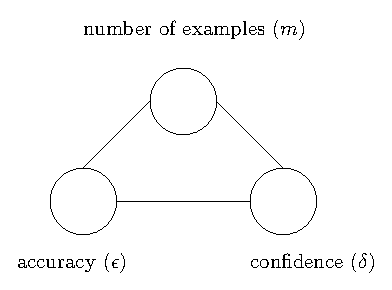
\includegraphics[scale=0.8]{chapters/pac/figures/connection_m_eps_delta.eps}
\end{figure}


\begin{figure}[h!]
	\centering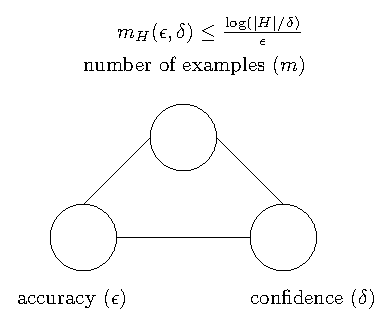
\includegraphics[scale=0.8]{chapters/pac/figures/connection_m_eps_delta_finite4.eps}
\end{figure}


\begin{figure}[h!]
	\centering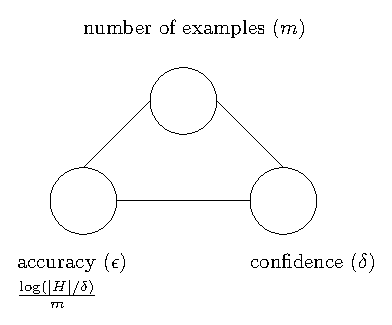
\includegraphics[scale=0.8]{chapters/pac/figures/connection_m_eps_delta_finite2.eps}
\end{figure}


\begin{figure}[h!]
	\centering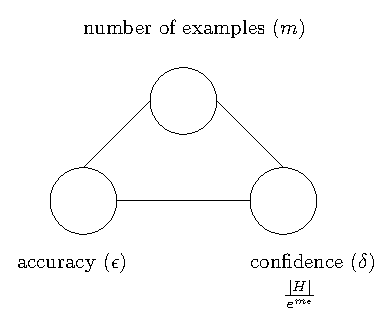
\includegraphics[scale=0.8]{chapters/pac/figures/connection_m_eps_delta_finite3.eps}
\end{figure}

To summarize this section, we have  the following:
{\bf A finite hypothesis class $\Hc$ is PAC learnable using the ERM learning algorithm, and has a sample complexity  $m_\Hc(\epsilon,\delta)\leq \log(|\Hc|/\delta)/\epsilon$ samples.}

%So, given $\epsilon,\delta \in (0,1)$, all that the learning algorithm needs is to be consistent with the sample (to be an ERM) while the sample size $m$ should satisfy $m\ge m_\Hc(\epsilon,\delta)= \frac{\log(|\Hc|/\delta)}{\epsilon}$.
Several natural questions may come to mind.

\begin{itemize}
	\item Is the bound $m_\Hc(\epsilon,\delta) \le \frac{\log(|\Hc|/\delta)}{\epsilon}$ tight? Can the ERM learner, or an other learner, be Probably Approximately correct (with accuracy $\epsilon$ and confidence $\delta$) using fewer than 
	$\frac{\log(|\Hc|/\delta)}{\epsilon}$ samples?
	\item What happens when noise is present so the $y$'s are not deterministically determined by $x$?
	\item What happens when our  hypothesis class is infinite?
\end{itemize}

Consider the last question. As we have seen,  the  class of threshold functions
over $\mathbb{R}$,  $\Hc_{th}$, in spite of being infinite, \textit{is}  PAC
learnable, with sample complexity $m_{\Hc_{th}}(\epsilon,\delta)
\le\frac{\log(1/\delta)}{\epsilon}$, which is obtained by using the
$ERM_{\Hc_{th}}$ learning rule. So  $\Hc_{th}$ appears to be simple to learn.
Can we explain why? Somehow, the hypothesis class $\Hc_{tr}$ is {\bf small} or
{\bf simple} and the hypothesis class $\Yc ^\Xc$ is {\bf large} or {\bf complicated}. 

What we need in order to answer the above questions systematically is some sort of a \textit{complexity measure} with which we can order classes by their difficulty along the complexity axis shown in the figure below.

\begin{figure}[h!]
	\centering
	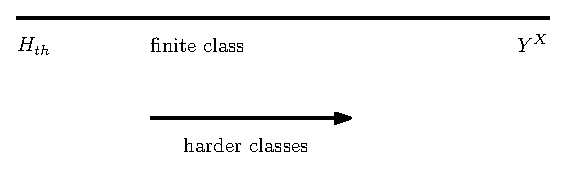
\includegraphics[scale=0.6]{chapters/pac/figures/complexity_measure.eps}
\end{figure}

For example, consider the \textbf{Two-Intervals} hypothesis class, defined by

\[\Xc = \R , \quad \Hc = \{ h_{a,b,c} : a < b < c \in \R \}\,,\]
where $h_{a,b,c}(x)=1$ if $x \in [a,b]$ or $x\geq c$ and $h_{a,b,c}(x)=0$ elsewhere.

\begin{figure}[h!]
	\centering
	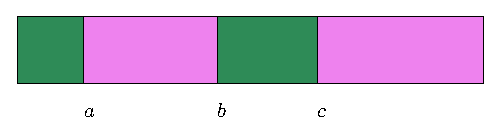
\includegraphics[scale=0.8]{chapters/pac/figures/2_intervals.eps}
\end{figure}



The following figures demonstrate this point. Suppose we would like to learn with threshold functions the following sample  (pink = 1, green = 0)
\begin{figure}[h!]
	\centering
	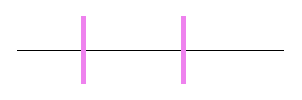
\includegraphics[scale=0.6]{chapters/pac/figures/VC_threshold_intuitive.eps}
\end{figure}

A possible answer would be:
\begin{figure}[h!]
	\centering
	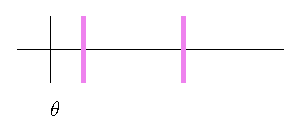
\includegraphics[scale=0.6]{chapters/pac/figures/VC_threshold_intuitive3.eps}
\end{figure}

However, if $x_1 < x_2$ and $y_1=1, y_2=0, $ can not be learned by $\Hc_{th}$, although it can be learned with 2-intervals:
\begin{figure}[h!]
	\centering
	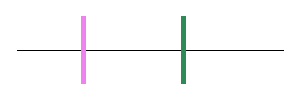
\includegraphics[scale=0.6]{chapters/pac/figures/VC_threshold_intuitive2.eps}
\end{figure}

\vspace{5mm}

\begin{figure}[h!]
	\centering
	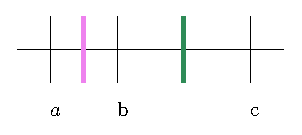
\includegraphics[scale=0.6]{chapters/pac/figures/VC_threshold_intuitive4.eps}
\end{figure}

Indeed, we somehow feel that the \textbf{2-Interval} class has larger complexity than that of $\Hc_{th}$ but smaller than that of finite classes.

\begin{figure}[h!]
	\centering
	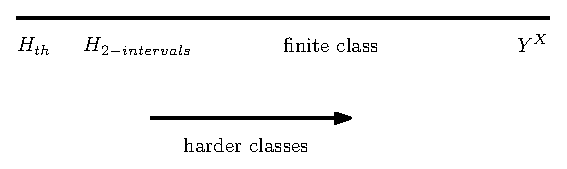
\includegraphics[scale=0.8]{chapters/pac/figures/complexity_measure2.eps}
\end{figure}

\section{VC Dimension}

VC-Dimension is the definition of complexity of an hypothesis class we are
looking for. This is a {\bf combinatorial measure of complexity} of a function
class. What does ``combinatorial measure'' mean here? It means that VC-dimension is just based on counting stuff, so that $\Xc$ can be any
set, with no additional structure. In particular, the VC-dimension of
$\Hc\subset \left\{ \pm 1 \right\}^\Xc$ is defined even if $\Xc$ does not need any
geometric or algebraic structure. VC-dimension is interesting as it provides a
decisive characterization of hypothesis classes that are "simple enough" to
learn (in the sense of PAC learnability), versus hypothesis classes that are "too complicated" to learn. It also provides a decisive characterization of $m_\Hc$, the sample complexity of a "simple" hypothesis class $\Hc$.  

\subsection{Motivation}

Suppose we got a training set $S = (x_1,y_1),\ldots,(x_m,y_m)$ and were able to fully explain the labels using a hypothesis from a class $\Hc$, namely, to find a function $h\in\Hc$ with empirical risk $L_S(h)=0$. Suppose that, only to see what will happen, we deliberately corrupt our sample $S$ by changing the labels $\{y_i\}$ - call the corrupt sample $S'$. Suppose that we  {\bf also} succeed in explaining $S'$  using a different hypothesis from the same class $\Hc$, namely, find another function $h'\in\Hc$ with $L_{S'}(h')=0$. If we can do that, no matter what corrupt labels we choose, it means that something isn't right: how can we hope to generalize based on a training sample $S$ if, regardless of the labels in $S$, we can find $h\in\Hc$ with $L_S(h)=0$? 
\vspace{3mm}
{\bf Definition:} Let $C\subset\Xc$ be a subset of the sample space and let $h:\Xc\to\Yc$ be some hypothesis. 
We define the {\bf restriction} of $h$ to $C$, denoted $h_C:C\to\Yc$, by $h_C(x)=h(x)$, for $x\in C$.
\vspace{3mm}
{\bf Here is a crucial observation:} Suppose that $\Hc$ contains {\bf all} functions over some set $C\subset\Xc$ of size $m$, in the sense that $\{h_C\,|\,h\in\Hc\} = (C\to\Yc)$. Then we cannot find a Probably Approximately correct learner that uses $m/2$ or fewer training samples.\\
Why? Go back to the "proof" of the No Free Lunch theorem we saw above. Suppose that indeed there exists a set $C\subset \Xc$ of size $m$ such that $\{h_C\,|\,h\in\Hc\} = (C\to\Yc)$. We play our game against Nature, choose a learner $\Ac$, and choose a training sample size of $m/2$ or less. Our learner specifies that if it hasn't seen a point $x\in\Xc$ in the training set, the output rule $h_S$ will predict $g(x)$ for some $g:\Xc\to\Yc$ we specify - we just make sure that the resulting $h_S$ will belong to $\Hc$. 
Now, as in the "proof" of the No Free Lunch theorem, Nature plays the distribution $\Dc$ that is uniform over  $C$, and makes an evil choice to play $f(x)=-g(x)$ for $x\in C$ (Since $\Dc$ is supported over $C$, Nature doesn't really care how her $f$ is defined outside $C$). {\bf This is a legal move for Nature since for every function $\tilde{f}:C\to\Xc$ there is a hypothesis $f\in\Hc$ with $f_C(x)=\tilde{f}(x)$, $x\in C$.} Again as in the "proof", our learner fails - regardless of the training sample of size $m/2$, the loss will be $1/2$.
\vspace{3mm}
We see that, as long as $\Hc$ contains {\bf any} set $C$ of size $2m$ with the property that $\{h_C\,|\,h\in\Hc\} = (C\to\Yc)$, then we cannot learn with a training sample of size $m$. It follows that the {\bf maximal size} of such a set $C$ in $\Hc$ is a {\bf critical quantity}: (i) it gives us a lower bound on $m_\Hc$, the minimal sample size needed, and (ii) if the maximal size is $\infty$, namely, if for any $m\in\mathbb{N} \Xc$ contains such as set $C$ with $|C|>m$, the $\Hc$ is not PAC-learnable!

\subsection{Formal Definition}

Let $C = \{x_1,\ldots,x_{|C|}\} \subset \Xc$ and let $\Hc_C$ be the restriction of $\Hc$ to $C$, namely,
$\Hc_C = \{ h_C : h \in \Hc\}$.
We are working with $\Yc=\{\pm 1\}$, so we can represent each $h_C$ as the vector $(h(x_1),\ldots,h(x_{|C|})) \in \{\pm 1\}^{|C|}$. Therefore the total number of possible such vectors is $2^{|C|}$, so that
$$|\Hc_C| \le 2^{|C|}\,.$$

We will say that $\Hc$ \textbf{shatters} $C$ if $|\Hc_C| =  2^{|C|}$.  
\begin{definition}
	The VC dimension of the hypothesis class $Hc$ is defined as 
	$$VCdim(\Hc) = \max\{ |C| ~:~ \Hc~\,\,\textrm{shatters}~\,\,C \}\,,$$
	that is, the VC dimension is the maximal size of a set $C\subset \Xc$ such that $\{h_C\,|\,h\in\Hc\} = (C\to\Yc)$.
\end{definition}
We interpret this as the maximal size of a set $C\subset X$ such that 
$\Hc$ gives no prior knowledge on label functions restricted to $C$.
%
\vspace{3mm}
According to the above definition, in order to show that $VCdim(\Hc) = d$ we need to show that:
\begin{enumerate}
	\item There exists a set $C$ of size $d$ which is shattered by $\Hc$.
	\item Every set $C$ of size $k$ with $k\geq d+1$ is not shattered by $\Hc$.
\end{enumerate}

\subsection{Exercises to help you understand the definition of VC-dimension}

Make sure to solve all these exercises. They will help you understand the
definition of VC-dimension.

\subsubsection{Axis aligned rectangles}
Consider the \textbf{Axis aligned rectangles} hypothesis class over the sample space 
$\Xc = \R ^2$. We define $\Hc = \{h_{(a_1,  a_2, b_1 , b_2)}: a_1 < a_2 ~\text{and}~  b_1 < b_2 \}$, 
where $ h_{(a_1, a_2, b_1 , b_2)}(x_1,x_2) = 1$ if $x_1 \in [a_1,a_2]$, and $x_2 \in [b_1,b_2]$, and  $ h_{(a_1, a_2, b_1 , b_2)}(x_1,x_2) = 0$ otherwise. (Convince yourself that a function in this hypothesis class is an indicator of a finite open rectangle aligned with the canonical basis of $\R ^2$.)

\vspace{9mm}

Verify that:
\begin{center}
	\begin{tabular}{lr}
		Shattered & Not Shattered \\
		\begin{tikzpicture}[scale=1]
			\fill[blue] (0,1) circle (0.1);
			\fill[blue] (1,0) circle (0.1);
			\fill[blue] (0,-1) circle (0.1);
			\fill[blue] (-1,0) circle (0.1);
		\end{tikzpicture} & \hspace{2cm}
		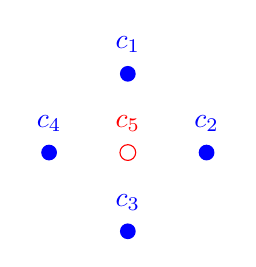
\begin{tikzpicture}[scale=1]
			\fill[blue] (0,1) circle (0.1) node[above=4pt] {$c_1$};
			\fill[blue] (1,0) circle (0.1) node[above=4pt] {$c_2$};
			\fill[blue] (0,-1) circle (0.1) node[above=4pt] {$c_3$};
			\fill[blue] (-1,0) circle (0.1) node[above=4pt] {$c_4$};
			\draw[red] (0,0) circle (0.1) node[above=4pt] {$c_5$};
		\end{tikzpicture}
	\end{tabular}
\end{center}
\vspace{3mm}
\begin{exercise}
	show that no set of 5 points can be shattered by the Axis aligned rectangles class. Hint: note that the 3 points $(x_k,y_k)$, $(x_i,y_i)$, and $(x_{k'},y_{k'})$ can not be shattered if $x_k\leq x_i\leq x_{k'}$ and $y_k\leq y_i\leq y_{k'}$.
\end{exercise} 


\subsubsection{Finite classes}
\begin{exercise}\
	\begin{itemize}
		\item Show that the VC dimension of a finite $\Hc$ is at most
		$\log_2(|\Hc|)$.
		\item  Assume $\Hc$ is finite. Show that there can be arbitrary gap between $VCdim(\Hc)$ and
		$\log_2(|\Hc|)$, namely, construct a finite hypothesis class $\Hc$ over some sample space $\Xc$ with $VCdim(\Hc) = \log_2(|\Hc|)$ 
		and another finite hypothesis class with $VCdim(\Hc)=1$.  
	\end{itemize}	
\end{exercise}


\subsubsection{Half-spaces through the origin}
Consider the sample space $\Xc = \R ^d$ and the hypothesis class of half-spaces through the origin
$\Hc = \{ \x \mapsto sign(\langle\w,\x \rangle ): \w \in \R ^d\}$. 

\begin{exercise}\
	\begin{itemize}
		\item Show that $ \{\mathbf{e}_1, ,\mathbf{e}_d \} $ is shattered 
		\item Show that any $d+1$ points cannot be shattered (hint: consider the standard basis vectors...)
		\item What is $VCdim(\Hc)$?
	\end{itemize}
	
\end{exercise}


%\subsubsection{Classification trees}
%What is the VC-dimension of a full balanced classification tree with $b$
%levels?

